%%%%%%%%%%%%%%%%%%%%%%%%%%%%%%%%%%%%%%%%%%%%%%
%                insertmeeting
% 1) Title (something creative & funny?)
% 2) Date (MM/DD/YYYY)
% 3) Location (ex. Hagerty High School)
% 4) People/Committees Present 
% 5) Picture 
% 6) Start Time & Stop Time (ex. 12:30AM to 4:30PM)
%%%%%%%%%%%%%%%%%%%%%%%%%%%%%%%%%%%%%%%%%%%%%%
\insertmeeting 
	{Team Time} 
	{08/10/21}
	{Hagerty High School}
	{Annika, Anouska, Clayton, Falon, James, Jensen, Nathan, Ritam, Rose, Samantha}
	{Images/RobotPics/robot.jpg}
	{2:20 - 4:30}
	
\hhscommittee{General}
\noindent\hfil\rule{\textwidth}{.4pt}\hfil
\subsubsection*{Goals}
\begin{itemize}
    \item Set up goals for the season
	\item Discuss GRPI model

\end{itemize} 

\noindent\hfil\rule{\textwidth}{.4pt}\hfil

\subsubsection*{Accomplishments}
At today's meeting, we went over the GRPI model --- a type of model that helps teams work together more effectively. GRPI stands for goals, roles, processes, and interpersonal relations. This model is designed to help teams asses and organize tasks. At this meeting, we started discussing our overall goals and creating a list of what each goal would entail (image 1) these goals encompassed everything we wanted to accomplish this season including having a fully functioning robot, having a well made notebook, reaching out to more professionals, expanding our outreach, creating an innovation project, and finally progressing to worlds. 
We also discussed our committees and what roles each of them would take. We used a chart organizing us into our main (blue) and secondary(gray) committees and allowed people to change their selections if desired (image 2). Additionally, we went over what each of these committees roles would be and what responsibilities its members would have, utilizing notes from a previous meeting and adding details and making changes where it was necessary(see images 3 and 4).

\begin{figure}[htp]
\centering
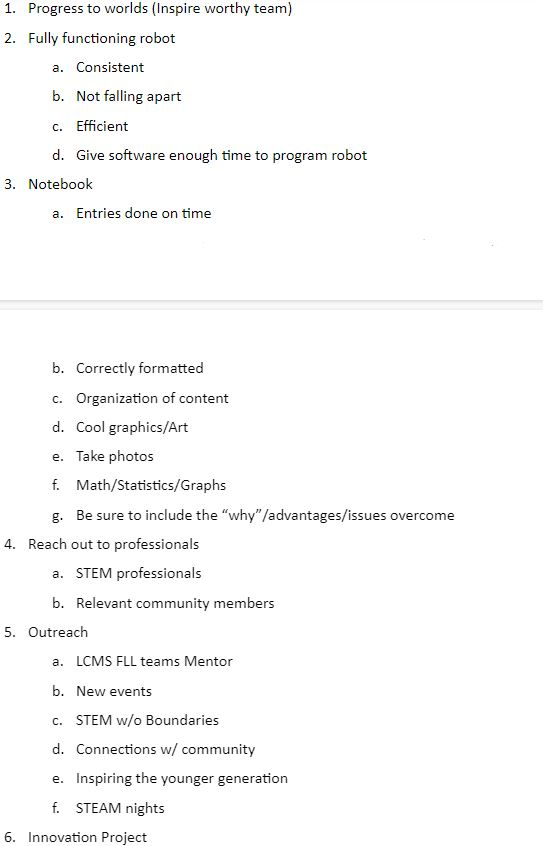
\includegraphics[width=0.9\textwidth, angle=0]{Meetings/August/08-10-21/8-10-21_Image1 - Nathan Forrer.JPG}
\caption{Plan for the season}
\label{fig:pic1}
\end{figure}

\begin{figure}[ht]
\centering
\begin{minipage}[b]{.48\textwidth}
	\centering
	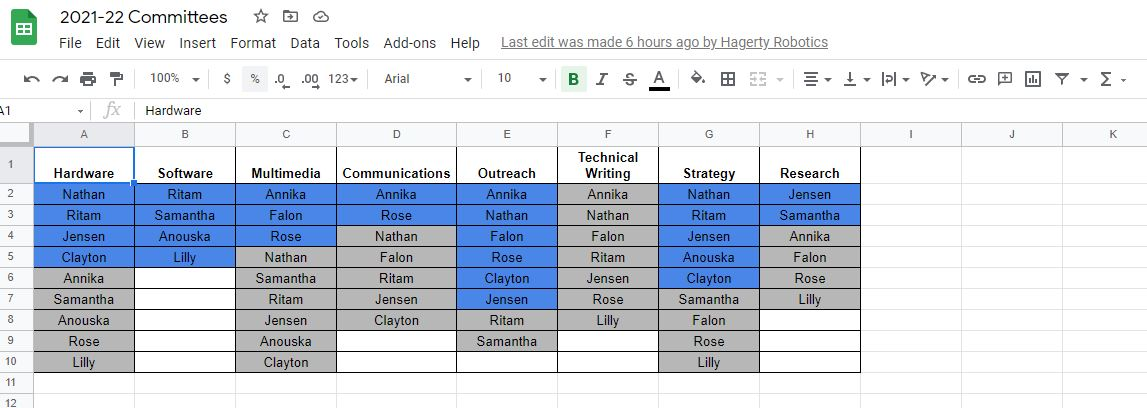
\includegraphics[width=0.95\textwidth, angle=0]{Meetings/August/08-10-21/8-10-21_Image2 - Nathan Forrer.JPG}
	\caption{Committee Division Sheet}
	\label{fig:pic2}
\end{minipage}%
\hfill%
\begin{minipage}[b]{.48\textwidth}
	\centering
	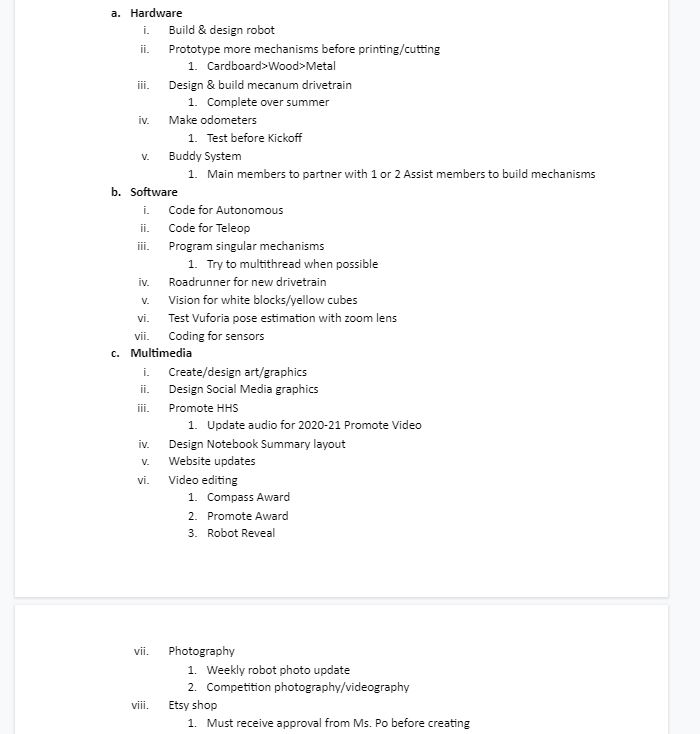
\includegraphics[width=0.95\textwidth, angle=0]{Meetings/August/08-10-21/8-10-21_Image3 - Nathan Forrer.JPG}
	\caption{Committee Goals Sheet}
	\label{fig:pic3}
\end{minipage}
\end{figure}

\begin{figure}[htp]
\centering
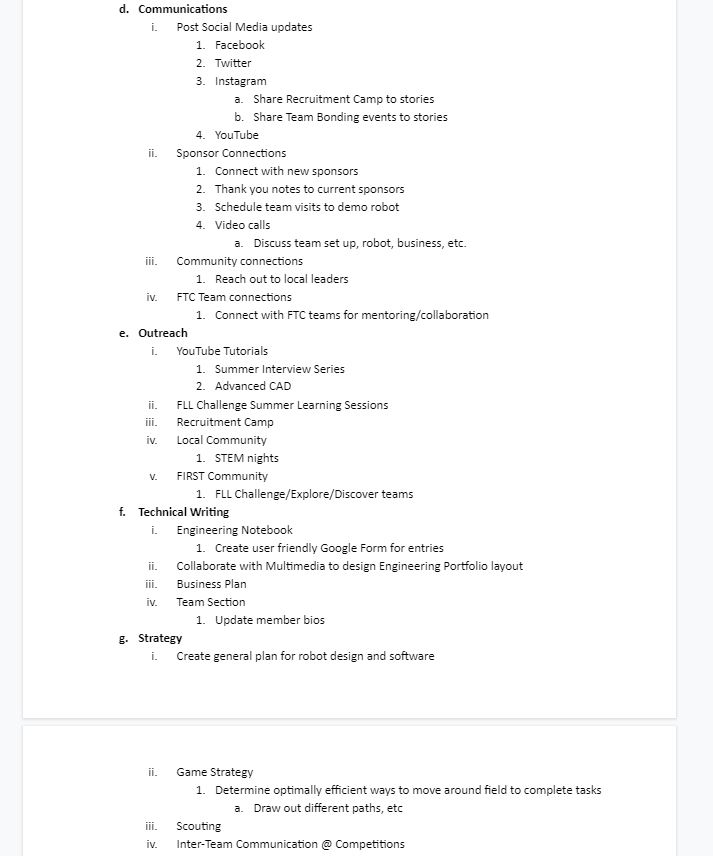
\includegraphics[width=0.9\textwidth, angle=0]{Meetings/August/08-10-21/8-10-21_Image4 - Nathan Forrer.JPG}
\caption{Committee Goals Sheet Continued}
\label{fig:pic4}
\end{figure}


\hhscommittee{Hardware}
\noindent\hfil\rule{\textwidth}{.4pt}\hfil
\subsubsection*{Goals}
\begin{itemize}
    \item Our meeting goals were to set up solid goals for the season. This set up a solid base line and allowed use to plan for the future. The process encouraged us to work backwards to better time manage. 
    \item start laser cutting rev hub holder
	\item teach newer members cad basics

\end{itemize} 

\noindent\hfil\rule{\textwidth}{.4pt}\hfil

\subsubsection*{Accomplishments}
During this meeting we set up goals for the beginning of the season, began cutting parts for adding on the control hub and battery, and we began programming a tele-op program. The cutting allowed use to have parts ready to assemble our robot. The programming will set us up for better driving and more time to work in the future. The goal planning encouraged backwards planning and how we need to move forwards.

To keep the team up to date we started the meeting with a review of the rev hub holder design. We began the construction of it today; we cut with the glowforge. The glowforge is slow so in the meantime we did a mini cad lesson to newer members. We started covering basic sketch and extrude tools, then advanced to the chamfer and fillet tools. As a test we had them attempt to sketch the first letter of their first name and scaffolded their learning

\hhscommittee{Multimedia}
\noindent\hfil\rule{\textwidth}{.4pt}\hfil
\subsubsection*{Goals}
\begin{itemize}
    \item We discussed the plans and goals for the upcoming season. We also planned and worked on finishing some tasks before kickoff

\end{itemize} 

\noindent\hfil\rule{\textwidth}{.4pt}\hfil

\subsubsection*{Accomplishments}
We discussed the plans for the upcoming season that we wanted to get done by kickoff. We updated our member bios on the website and for the 2021-22 season notebook. 